% 聚类算法对比实验主体章节
\chapter{聚类算法对比实验}

\section{实验目标}
本章在鸢尾花（Iris）数据集上实现并比较两种常用的无监督聚类算法：手写实现的 \textbf{K-means} 与 \textbf{DBSCAN}。重点内容包括：
\begin{itemize}
    \item 手写实现两种算法的核心逻辑（禁止直接使用 sklearn 的聚类实现）；
    \item 通过调整超参数（K-means 的 $k$，DBSCAN 的 $\varepsilon$ 与 $\mathrm{min\_samples}$）观察聚类结果变化；
    \item 使用准确率（需对齐簇标签）、轮廓系数与 Calinski-Harabasz 指数对聚类性能进行评估；
    \item 将结果以表格与可视化图像展示，并在报告中分析和讨论。
\end{itemize}

\section{数据集与预处理}
本实验使用 sklearn 提供的鸢尾花（Iris）数据集。数据包含 $n=150$ 个样本，每个样本有 $d=4$ 个数值特征：萼片长度、萼片宽度、花瓣长度、花瓣宽度；并带有 3 类真实标签（Setosa、Versicolor、Virginica）。

预处理步骤如下：
\begin{enumerate}
    \item 缺失值检查：原数据无缺失值，直接使用；
    \item 特征标准化：对每一维特征做 Z-score 标准化，公式为
    $$x' = \frac{x-\mu}{\sigma},$$
    其中 $\mu$、$\sigma$ 分别为该维度的样本均值与标准差；标准化可以避免不同量纲对距离计算的影响；
\end{enumerate}

\section{算法原理}
\subsection{K-means 原理}
K-means 试图将样本划分为 $k$ 个簇，使得簇内方差最小化。定义簇标签 $z_i\in\{1,\dots,k\}$，簇中心为 $\mu_j$，优化目标为：
$$\min_{z,\{\mu_j\}} \; J = \sum_{i=1}^n ||x_i - \mu_{z_i}||^2.$$ 
给定簇分配时，最优质心为每簇点的均值：
$$\mu_j = \frac{1}{|C_j|}\sum_{i\in C_j} x_i.$$ 
交替优化（E-step：按最近中心分配；M-step：按簇均值更新中心）会使目标函数单调下降并在有限步内收敛到局部极小点。K-means 对初始中心敏感，常用多次随机初始化取最优解。

\subsection{DBSCAN 原理}
DBSCAN 基于密度的聚类思想：
\begin{itemize}
    \item 对每个点 $p$，其 $\varepsilon$-邻域定义为 $N_\varepsilon(p)=\{q: ||q-p||\le\varepsilon\}$；
    \item 若 $|N_\varepsilon(p)|\ge\mathrm{min\_samples}$，则 $p$ 为\textbf{核心点}；
    \item 核心点之间若可达（通过核心点链），则属于同一簇；非核心但位于某核心点邻域内的点为\textbf{边界点}；既非核心也不在任何核心邻域内的点为\textbf{噪声}。 
\end{itemize}
DBSCAN 无需预先指定簇数，可发现任意形状簇并自动识别离群点，但对 $\varepsilon$ 与 $\mathrm{min\_samples}$ 敏感。

\section{核心算法伪代码}
\subsection{K-means}
K-means 的基本流程为：随机初始化 $k$ 个质心，重复进行样本到质心的最近邻分配与质心重计算，直至收敛。

\begin{lstlisting}[style=cleanpython]
Input: X (n x d), k, max_iters, tol
Initialize centroids C by sampling k points from X
for t in range(max_iters):
    for each sample i: assign label[i] = argmin_j ||X[i]-C[j]||
    for each cluster j: C_new[j] = mean of members
    if ||C_new - C|| < tol: break
    C = C_new
return labels, C
\end{lstlisting}

\subsection{DBSCAN}
DBSCAN 通过密度连接定义簇：对于每个点，若其 $\varepsilon$ 邻域内点数不小于 $\mathrm{min\_samples}$，则为核心点并扩展簇。
\begin{lstlisting}[style=cleanpython]
Input: X, eps, min_samples
labels = UNVISITED
cluster_id = 0
for each point p:
    if p is visited: continue
    N = neighbors(p, eps)
    if |N| < min_samples: labels[p] = NOISE
    else:
        labels[p] = cluster_id
        seeds = N \ {p}
        for q in seeds:
            if q is NOISE: labels[q] = cluster_id
            if q not visited:
                labels[q] = cluster_id
                Nq = neighbors(q, eps)
                if |Nq| >= min_samples: seeds += Nq
        cluster_id += 1
return labels
\end{lstlisting}

上述指标均在代码中手写实现，没有使用 sklearn 的现成库。


\section{参数设置与实验设计}
\begin{itemize}
    \item K-means: 测试 $k=2,3,4,5$；随机种子固定以便复现。
    \item DBSCAN: 测试 $\varepsilon=\{0.3,0.5,0.8,1.0\}$ 与 $\mathrm{min\_samples}=\{3,5,7\}$。
    \item 对每组参数记录：Accuracy（对齐簇标签后）、Silhouette、Calinski-Harabasz 及噪声点数（DBSCAN）。
\end{itemize}

\section{评估指标设计与实现}
本次实验采用三类指标评估聚类效果：
\begin{enumerate}
    \item \textbf{Accuracy（准确率，需标签对齐）}：聚类是无监督的，簇标签与真实标签无对应关系。我们通过标签对齐（枚举映射或匈牙利算法）找到使匹配数量最大的映射 $\pi$，Accuracy 定义为
    $$\mathrm{Accuracy} = \frac{1}{n} \sum_{i=1}^n \mathbf{1}\{\pi(\hat{y}_i)=y_i\}.$$ 

    \item \textbf{轮廓系数（Silhouette）}：对每个样本 $i$，令 $a(i)$ 为该样本与同簇其他点的平均距离，$b(i)$ 为其到最近异簇点的平均距离，则样本的轮廓系数为
    $$s(i)=\frac{b(i)-a(i)}{\max\{a(i),b(i)\}}\in[-1,1].$$
    整体轮廓系数为所有样本 $s(i)$ 的平均值（噪声点在计算时可按 0 处理或忽略，本实现忽略标签为 $-1$ 的噪声点）。该指标兼顾簇内紧密度与簇间分离度。

    \item \textbf{Calinski-Harabasz 指数（CH）}：基于簇间和簇内方差比率定义，计算公式为
    $$\mathrm{CH}=\frac{\mathrm{trace}(B)/(k-1)}{\mathrm{trace}(W)/(n-k)}=\frac{\mathrm{between}/(k-1)}{\mathrm{within}/(n-k)},$$
    其中 $\mathrm{between}=\sum_{j} n_j ||\mu_j - \mu||^2$，$\mathrm{within}=\sum_j \sum_{i\in C_j} ||x_i-\mu_j||^2$，$\mu$ 为样本总体均值，$n_j$ 为簇 $j$ 大小。CH 指数越大，说明簇间差异越显著、簇内越紧凑。
\end{enumerate}

上述指标均在代码中手写实现，避免使用 sklearn 的现成度量函数。

\section{实验结果}
\subsection{K-means 结果}
下表给出 K-means 在不同 $k$ 下的评估结果：
\begin{table}[htbp]
    \centering
    \caption{K-means 不同 $k$ 下的评估结果}
    \label{tab:kmeans_results}
    \begin{tabular}{|c|c|c|c|}
        \hline
        $k$ & Accuracy & Silhouette & Calinski-Harabasz \\
        \hline
        2 & 0.6667 & 0.5818 & 251.3493 \\
        3 & 0.8533 & 0.4565 & 239.4845 \\
        4 & 0.6467 & 0.4151 & 206.2286 \\
        5 & 0.3733 & 0.3965 & 171.3978 \\
        \hline
    \end{tabular}
\end{table}

\subsection{DBSCAN 结果}

表中呈现 DBSCAN 多组参数结果，并给出噪声点数：
\begin{table}[htbp]
    \centering
    \caption{DBSCAN 参数组合结果}
    \label{tab:dbscan_results}
    \begin{tabular}{|c|c|c|c|c|c|}
        \hline
        $\varepsilon$ & $\mathrm{min\_samples}$ & Accuracy & Silhouette & CH & Noise \\
        \hline
        0.3 & 3 & 0.12 & 0.3974 & 564.8942 & 84 \\
        0.3 & 5 & 0.12 & 0.6302 & 4169.2823 & 120 \\
        0.3 & 7 & 0.08 & 0.6276 & 11827.2833 & 129 \\
        0.5 & 3 & 0.5733 & 0.2591 & 90.4069 & 17 \\
        0.5 & 5 & 0.56 & 0.6559 & 458.5748 & 34 \\
        0.5 & 7 & 0.52 & 0.4360 & 261.2142 & 46 \\
        0.8 & 3 & 0.66 & 0.5979 & 285.6262 & 4 \\
        0.8 & 5 & 0.66 & 0.5979 & 285.6262 & 4 \\
        0.8 & 7 & 0.6467 & 0.6065 & 306.0209 & 7 \\
        1.0 & 3 & 0.66 & 0.5868 & 258.6397 & 1 \\
        1.0 & 5 & 0.66 & 0.5952 & 278.9375 & 3 \\
        1.0 & 7 & 0.66 & 0.5952 & 278.9375 & 3 \\
        \hline
    \end{tabular}
\end{table}

\subsection{可视化结果对比}
% 并排展示 K-means 与 DBSCAN 的可视化结果
\begin{figure}[htbp]
    \centering
    \begin{subfigure}[t]{0.48\textwidth}
        \centering
        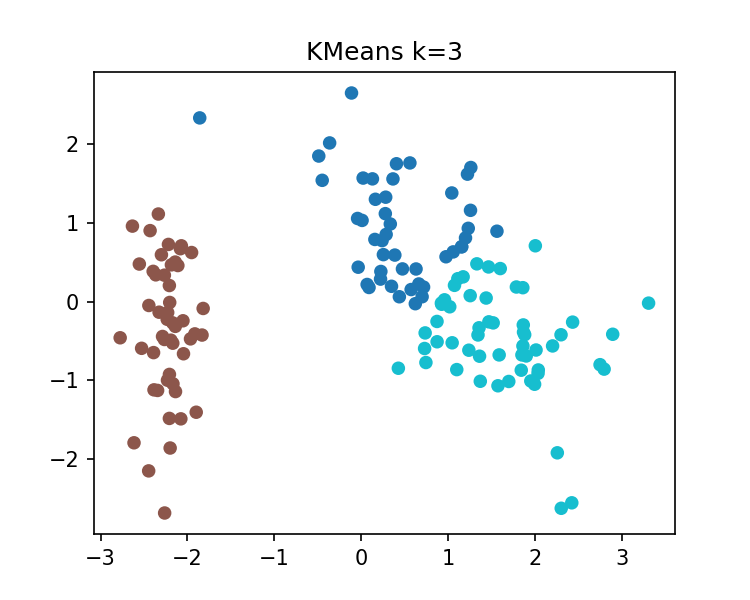
\includegraphics[width=\textwidth]{code/plots/kmeans_k3.png}
        \caption{K-means 聚类结果（$k=3$）}
        \label{fig:kmeans_k3}
    \end{subfigure}\hfill
    \begin{subfigure}[t]{0.48\textwidth}
        \centering
        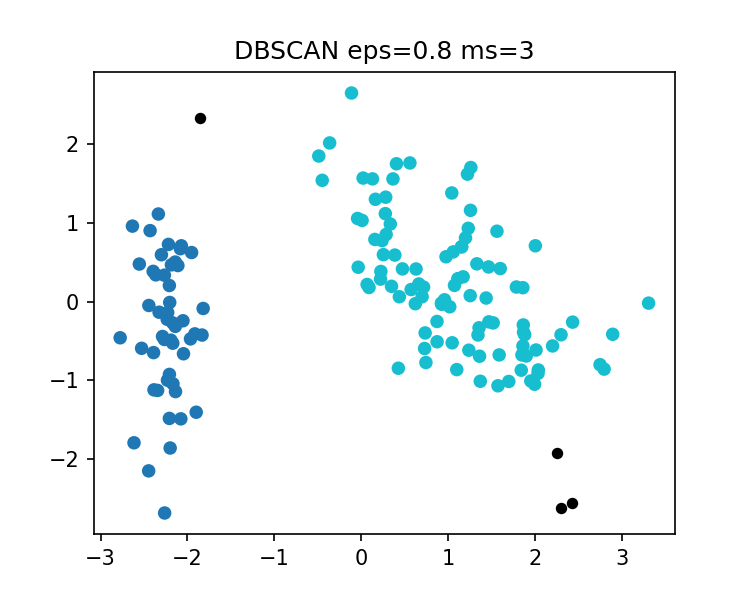
\includegraphics[width=\textwidth]{code/plots/dbscan_eps0.8_ms3.png}
        \caption{DBSCAN 聚类结果（$\varepsilon=0.8$, $\mathrm{min\_samples}=3$）}
        \label{fig:dbscan_best}
    \end{subfigure}
    \caption{K-means 与 DBSCAN 聚类结果对比（PCA 2D 投影）}
    \label{fig:kmeans_dbscan_compare}
\end{figure}

\subsection{全部实验可视化一览}
在此处将所有预先设置 K-means 参数的结果以及 DBSCAN 所有参数组合的结果全部展示出来。

\begin{figure}[htbp]
    \centering
    \begin{minipage}{0.24\textwidth}\centering
        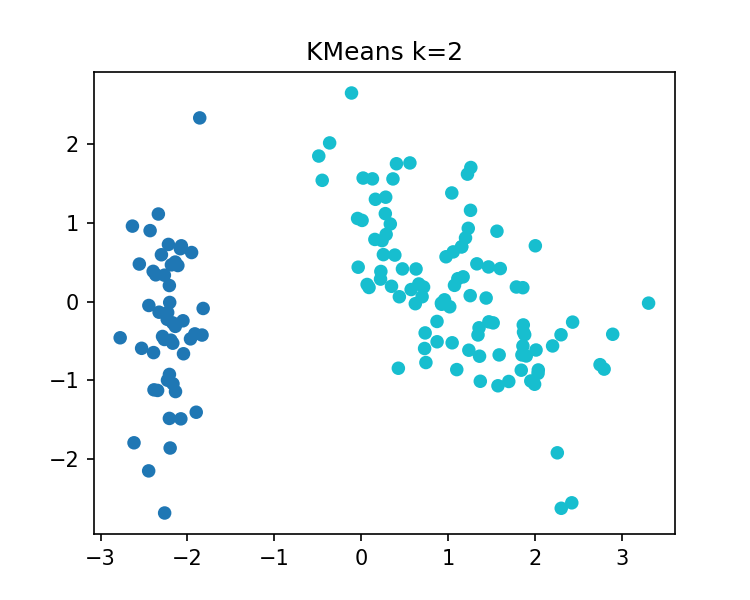
\includegraphics[width=\textwidth]{code/plots/kmeans_k2.png}
        \caption*{K=2}
    \end{minipage}\hfill
    \begin{minipage}{0.24\textwidth}\centering
        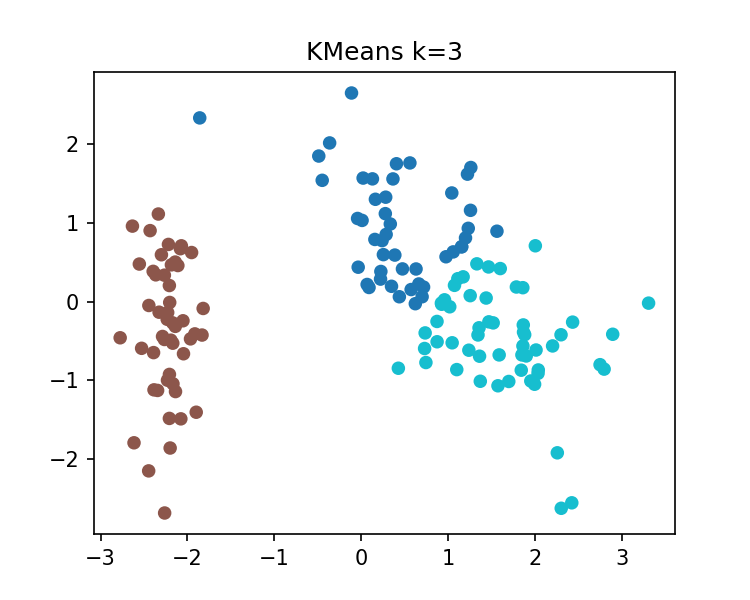
\includegraphics[width=\textwidth]{code/plots/kmeans_k3.png}
        \caption*{K=3}
    \end{minipage}\hfill
    \begin{minipage}{0.24\textwidth}\centering
        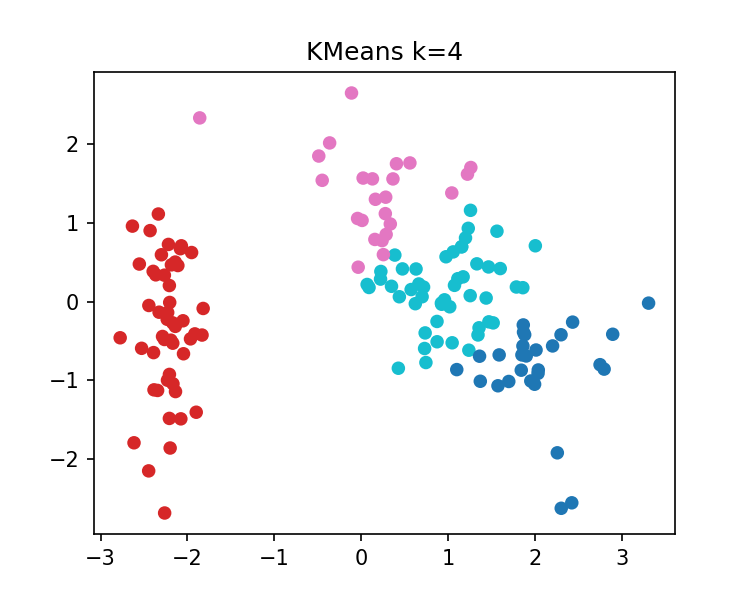
\includegraphics[width=\textwidth]{code/plots/kmeans_k4.png}
        \caption*{K=4}
    \end{minipage}\hfill
    \begin{minipage}{0.24\textwidth}\centering
        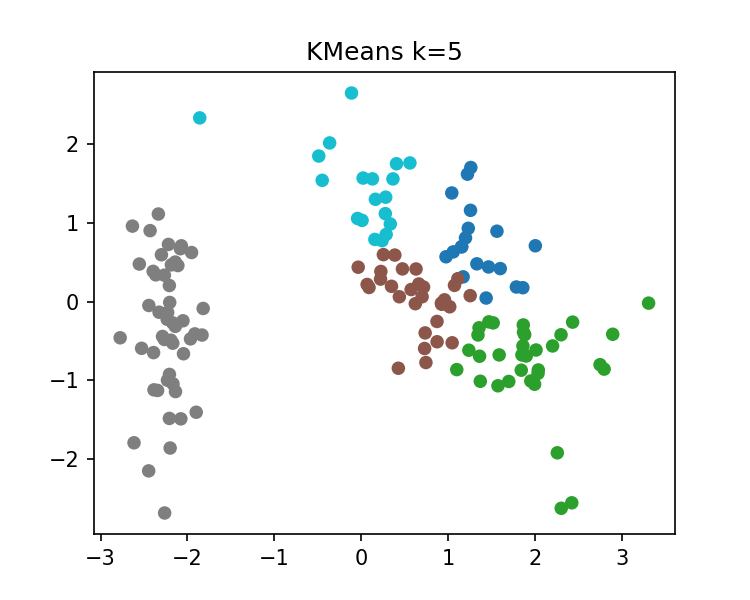
\includegraphics[width=\textwidth]{code/plots/kmeans_k5.png}
        \caption*{K=5}
    \end{minipage}
    \caption{K-means 在不同 $k$ 下的 PCA 可视化（四图并列）}
    \label{fig:kmeans_grid}
\end{figure}

\begin{figure}[htbp]
    \centering
    % row 1: eps=0.3
    \begin{minipage}{0.24\textwidth}\centering
        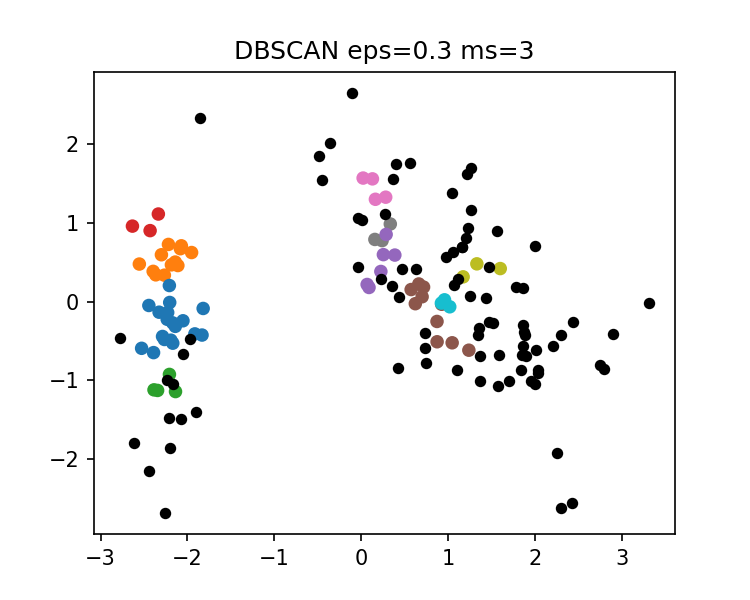
\includegraphics[width=\textwidth]{code/plots/dbscan_eps0.3_ms3.png}\caption*{$\varepsilon=0.3,\;m=3$}
    \end{minipage}\hfill
    \begin{minipage}{0.24\textwidth}\centering
        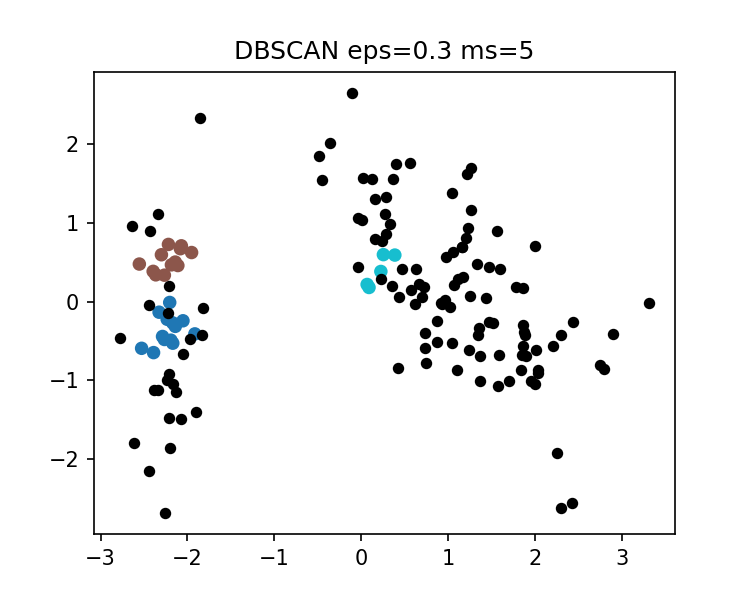
\includegraphics[width=\textwidth]{code/plots/dbscan_eps0.3_ms5.png}\caption*{$\varepsilon=0.3,\;m=5$}
    \end{minipage}\hfill
    \begin{minipage}{0.24\textwidth}\centering
        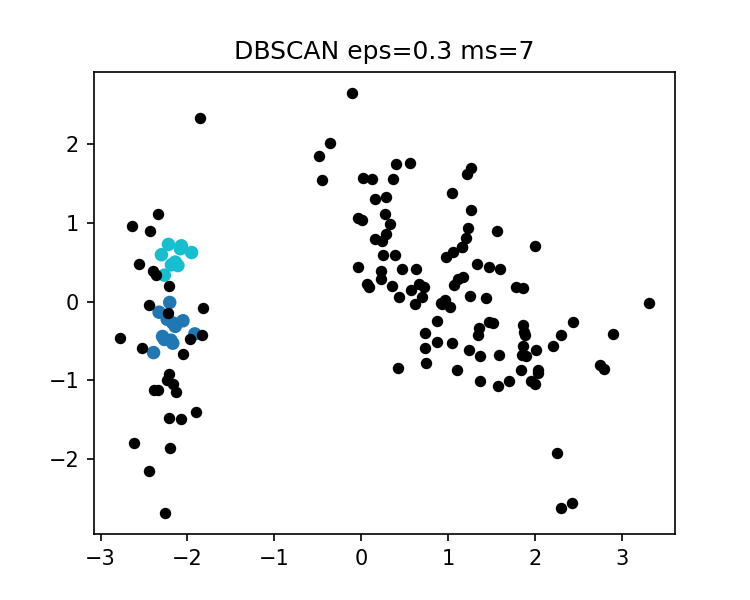
\includegraphics[width=\textwidth]{code/plots/dbscan_eps0.3_ms7.png}\caption*{$\varepsilon=0.3,\;m=7$}
    \end{minipage}\hfill
    \begin{minipage}{0.24\textwidth}\centering
        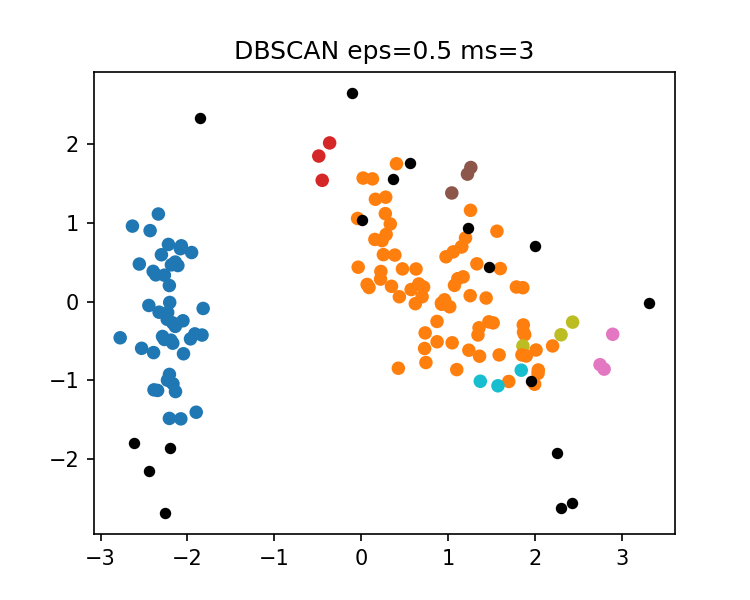
\includegraphics[width=\textwidth]{code/plots/dbscan_eps0.5_ms3.png}\caption*{$\varepsilon=0.5,\;m=3$}
    \end{minipage}

    % row 2: eps=0.5 cont
    \vspace{0.5em}
    \begin{minipage}{0.24\textwidth}\centering
        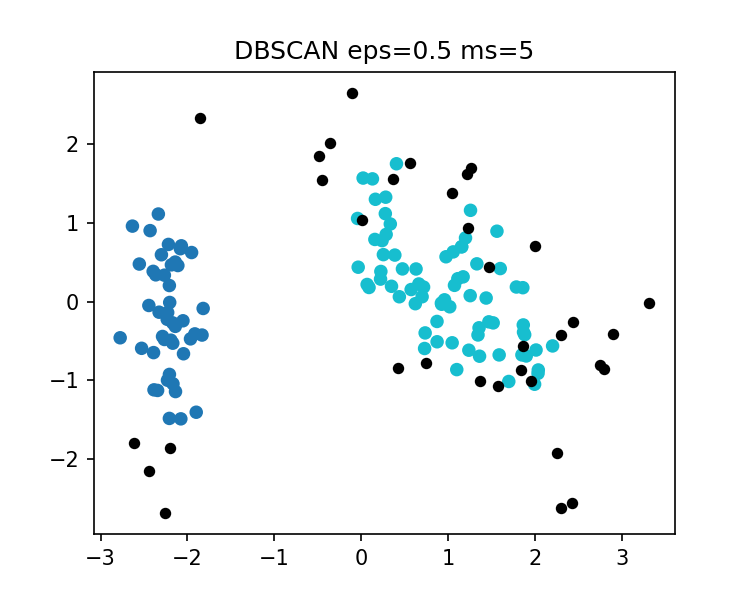
\includegraphics[width=\textwidth]{code/plots/dbscan_eps0.5_ms5.png}\caption*{$\varepsilon=0.5,\;m=5$}
    \end{minipage}\hfill
    \begin{minipage}{0.24\textwidth}\centering
        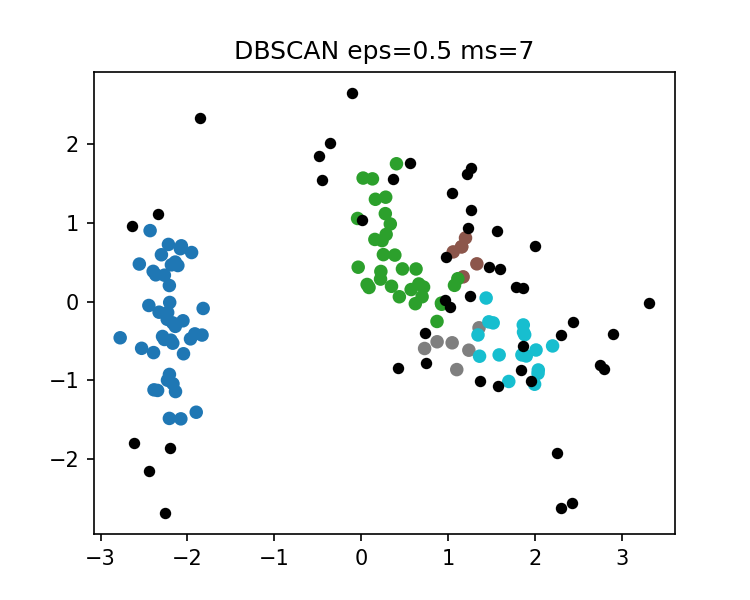
\includegraphics[width=\textwidth]{code/plots/dbscan_eps0.5_ms7.png}\caption*{$\varepsilon=0.5,\;m=7$}
    \end{minipage}\hfill
    \begin{minipage}{0.24\textwidth}\centering
        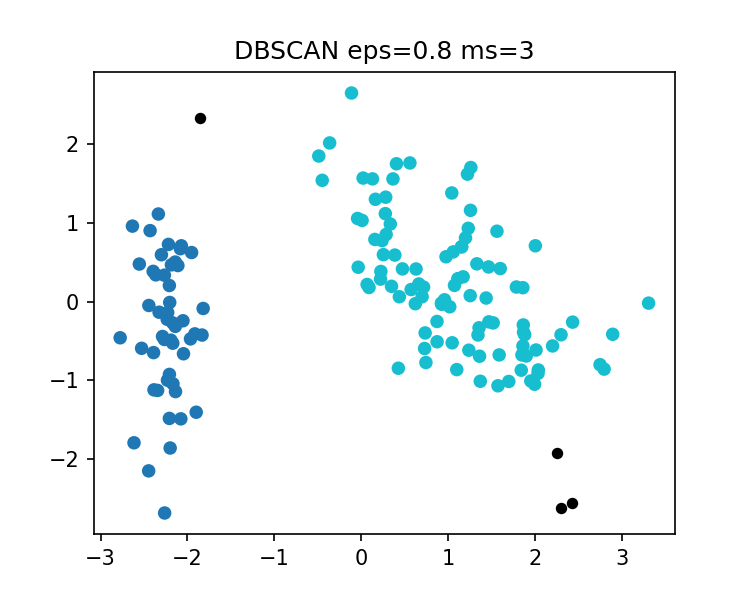
\includegraphics[width=\textwidth]{code/plots/dbscan_eps0.8_ms3.png}\caption*{$\varepsilon=0.8,\;m=3$}
    \end{minipage}\hfill
    \begin{minipage}{0.24\textwidth}\centering
        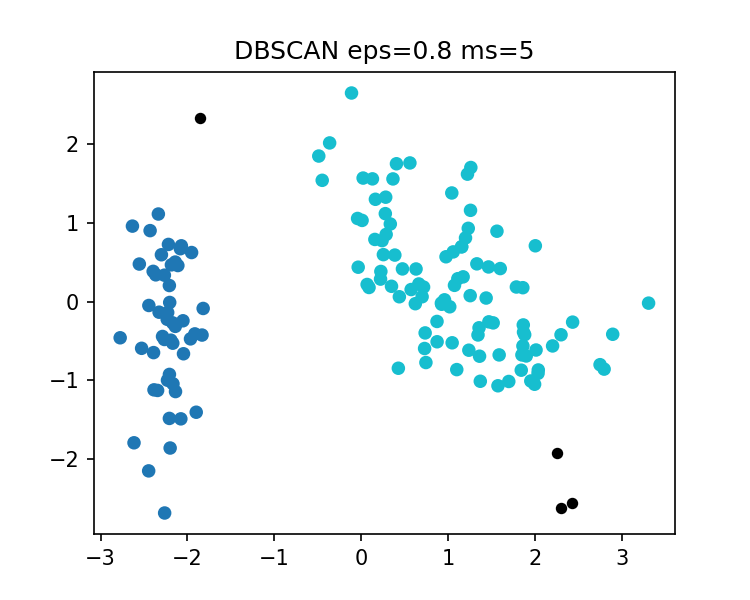
\includegraphics[width=\textwidth]{code/plots/dbscan_eps0.8_ms5.png}\caption*{$\varepsilon=0.8,\;m=5$}
    \end{minipage}

    % row 3: eps=0.8 cont & eps=1.0
    \vspace{0.5em}
    \begin{minipage}{0.24\textwidth}\centering
        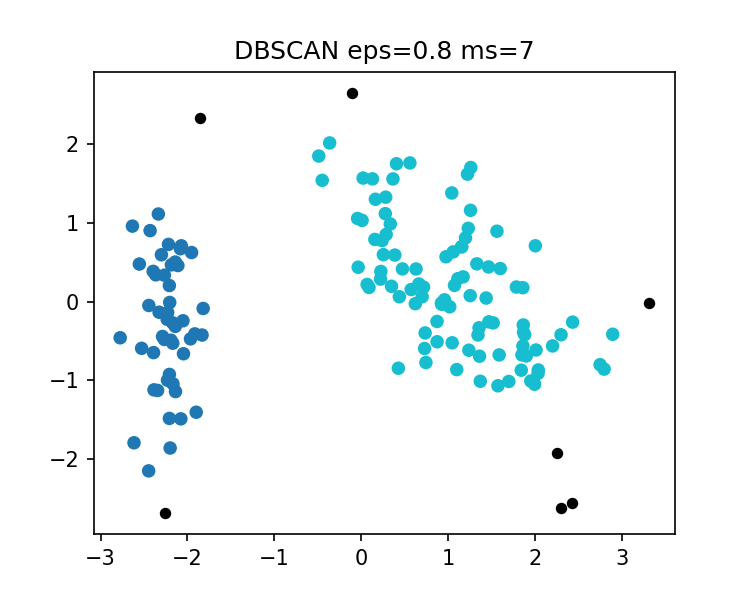
\includegraphics[width=\textwidth]{code/plots/dbscan_eps0.8_ms7.png}\caption*{$\varepsilon=0.8,\;m=7$}
    \end{minipage}\hfill
    \begin{minipage}{0.24\textwidth}\centering
        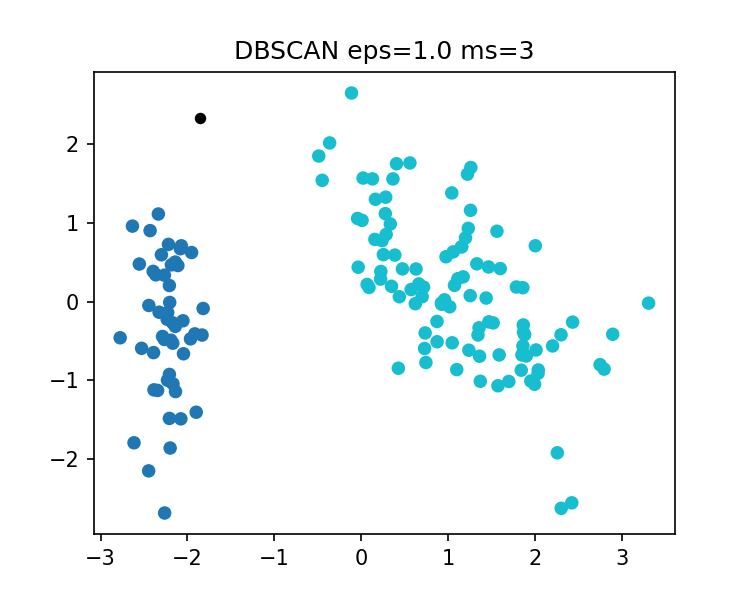
\includegraphics[width=\textwidth]{code/plots/dbscan_eps1.0_ms3.png}\caption*{$\varepsilon=1.0,\;m=3$}
    \end{minipage}\hfill
    \begin{minipage}{0.24\textwidth}\centering
        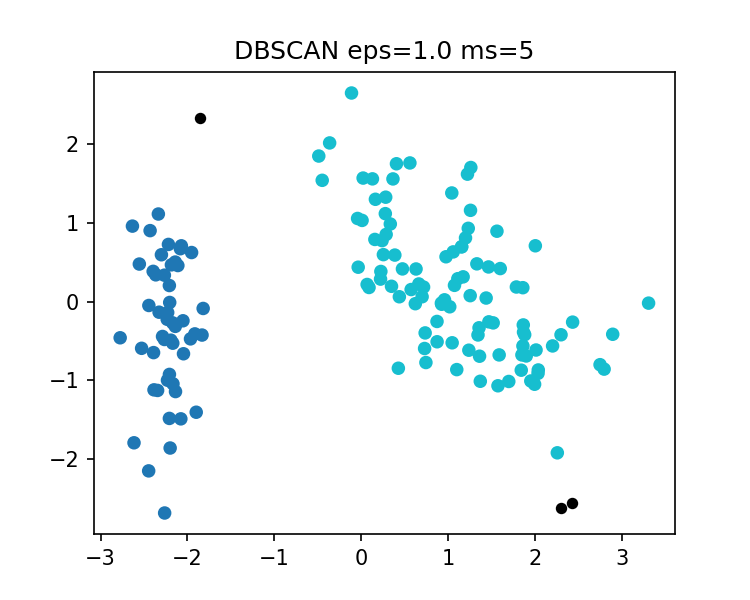
\includegraphics[width=\textwidth]{code/plots/dbscan_eps1.0_ms5.png}\caption*{$\varepsilon=1.0,\;m=5$}
    \end{minipage}\hfill
    \begin{minipage}{0.24\textwidth}\centering
        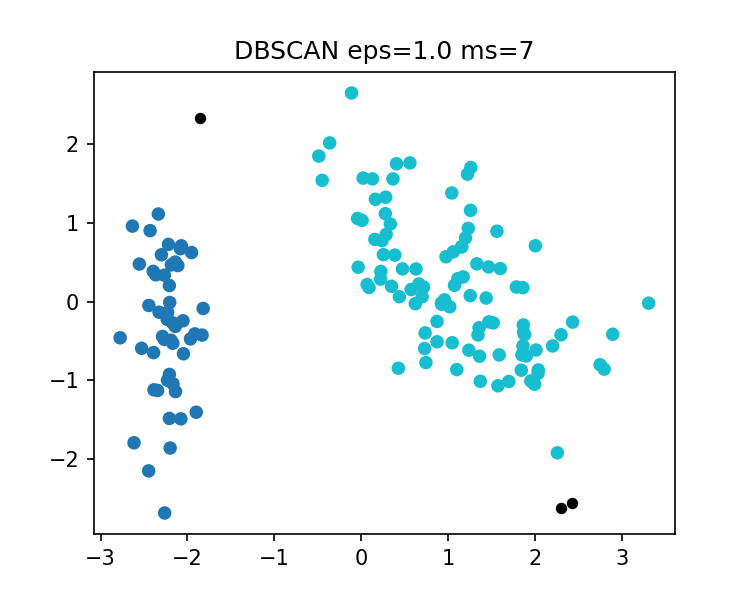
\includegraphics[width=\textwidth]{code/plots/dbscan_eps1.0_ms7.png}\caption*{$\varepsilon=1.0,\;m=7$}
    \end{minipage}

    \caption{DBSCAN 在所有参数组合下的聚类可视化（PCA 2D，4 列 x 3 行）}
    \label{fig:dbscan_all}
\end{figure}


\section{实验结果分析与评价}
\subsection{实验结果分析}
\begin{itemize}
    \item 从表 \ref{tab:kmeans_results} 可见，当 $k=3$ 时 K-means 的 Accuracy 达到最高（0.8533），这与鸢尾花数据集本身的三类结构一致，说明 K-means 在簇为凸且大小相近时表现较好。
    \item 轮廓系数在 $k=2$ 时最高（0.5818），这是因为把某两类合并后簇内紧密度提升，但 Accuracy 并非最优；因此不同指标反映聚类质量的侧重点不同，应同时考量。
    \item DBSCAN 在合适参数下（例如 $\varepsilon=0.8$, $\mathrm{min\_samples}=3$）能达到较高的 Accuracy（0.66）且噪声点少（4 个），说明其能够发现非球形簇与剔除离群点，但对参数较为敏感（见表 \ref{tab:dbscan_results}）。
    \item Calinski-Harabasz 指数在某些 DBSCAN 参数下异常较大（例如 $\varepsilon=0.3$ 且 $\mathrm{min\_samples}$ 较大时），这通常由于大量点被标记为噪声或簇数极少导致簇间/簇内方差比例异常，应结合其它指标与可视化共同判断。
\end{itemize}

\subsection{实验结果评价}
本节结合实验设计与上表/可视化结果对两种算法的性能、适用性与参数敏感性给出评价与建议。

\begin{itemize}
    \item \textbf{K-means 性能与适用性}：实验中 K-means 在 $k=3$ 时取得最高 Accuracy（0.8533），说明在鸢尾花数据上簇数 $k=3$ 与真实类别一致时模型能较好恢复类标。K-means 的 Silhouette 在 $k=2$ 更高（0.5818），这表明在二维 PCA 投影上合并两类可获得更紧密的簇内结构，但从分类匹配角度并非最优。综上：当关注“恢复真实类别”时优先选择与先验一致的 $k$；当关注簇内部结构紧密度与可分性时可结合 Silhouette 指标选择 $k$。

    \item \textbf{DBSCAN 的表现与参数敏感性}：DBSCAN 在不同 $\varepsilon$ 与 $\mathrm{min\_samples}$ 下表现差异显著。较小的 $\varepsilon$（如 0.3）会将大量点标记为噪声，导致 CH 指数异常增大（由于有效簇数很少且簇间方差/簇内方差比率失衡），Accuracy 同样偏低；而 $\varepsilon=0.8$ 且 $\mathrm{min\_samples}=3$ 时既能保持较少的噪声点（4 个），又能取得较高的 Silhouette 与合理的 Accuracy（0.66）。因此对 DBSCAN 建议通过参数扫描并结合可视化与噪声比例来选择参数，或使用 kNN 距离曲线（Elbow 法）辅助确定 $\varepsilon$。

    \item \textbf{指标冲突的理解与实用建议}：Accuracy、Silhouette 与 CH 指数各有侧重点：
    \begin{itemize}
        \item Accuracy 评估聚类结果与真实标签的一致性，依赖于类别对齐；适合有监督参考时使用；
        \item Silhouette 更关注簇内紧密度与簇间分离度，适合无监督质量判断；
        \item CH 指数对簇数量及簇大小敏感，在存在大量噪声或极不平衡簇时可能出现异常值。
    \end{itemize}
    因此在选择模型与参数时，推荐同时参考三者并结合 PCA 可视化结果，而非单一指标。

    \item \textbf{鲁棒性与复现性}：当前实验为一次性运行的结果，存在随机初始化与噪声导致波动的风险。实用建议：对 K-means 进行多次随机初始化（例如 10 次）并取最小 SSE/最大 CH 的结果；对 DBSCAN 在邻域参数附近做更细粒度扫描并统计噪声比例的稳定性。
\end{itemize}

\chapter{总结}

\section{实验总结}
本实验在鸢尾花（Iris）数据集上实现并对比了手写的 K-means 与 DBSCAN 两种聚类算法。主要结论如下：

1. K-means 在 $k=3$ 时取得最佳分类一致性（Accuracy = 0.8533），在簇为凸且大小相近的场景表现良好；
2. DBSCAN 在 $\varepsilon=0.8$、$\mathrm{min\_samples}=3$ 时取得较为平衡的结果（Accuracy 约为 0.66，噪声点 4 个），但对参数敏感；
3. 综合 Accuracy、Silhouette 与 Calinski–Harabasz 指数及可视化可知：K-means 适合球形、簇数已知或可近似估计的场景，DBSCAN 更适合发现任意形状簇并能自动识别离群点，但需细调参数。

基于以上结果分析，可以对 K-means 使用多次随机初始化并取最优解；对 DBSCAN 在参数附近进行更细粒度的扫描并结合 kNN 距离曲线辅助选取 $\varepsilon$。

\section{技术学习总结}
通过本次实验，我在以下几方面有明显收获：
\begin{itemize}
    \item 深入理解并手写实现 K-means 与 DBSCAN 的核心流程与边界情形（如空簇处理、噪声点标识与簇扩展逻辑）；
    \item 掌握了聚类评估指标的含义与计算：Accuracy 的标签对齐方法、Silhouette 系数与 Calinski–Harabasz 指数的计算与适用场景；
    \item 强化了实验设计与复现性实践，包括参数网格搜索、随机种子控制、多次试验统计与结果可视化实践（PCA 投影）；
\end{itemize}

\section{心得体会}
本次作业强化了我对无监督学习方法原理与工程实现的理解。体会到参数敏感性是聚类方法的核心挑战之一，单一评价指标往往不足以全面反映聚类质量，因此需要结合多种指标和可视化结果进行判断。后续可在更多数据集上做稳定性测试，或尝试混合基于距离与密度的算法以提升鲁棒性。

